\chapter{Developing for Android}
\label{chap:android}

Android, Inc\@. was founded in October in 2003 by Andy Rubin, Rich Miner, Nick Sears, and Chris White. 
At first, the company planned to develop an operating system for digital cameras % but when they realised that the market is not large enough,
but ultimately % they decided to change their intentions and 
decided to focus on smartphones instead. % operating system.
% That time, the Apple's iPhone was not released yet. 
% The rival mobile phones operating systems were Symbian and Windows Mobile.
% After four years with the financial aid of Google, Android was revealed.
HTC Dream, the first phone with the Android operating system, was sold in autumn 2008.
Majority of Android's code is released under a free license. 
This allows developers to modify and (with certain exceptions) freely distribute the software.
Due to this, Android became the most popular operating system for smartphones.
In this chapter, we introduce this system from programmer's perspective and give a brief description of how to implement an Android application.
The purpose of the chapter is to highlight the main architectural differences of Android and conventional desktop platforms rather then providing a complete programer's manual. 

\section{Introduction to the Android development}

Android is a product of \term{The Open Handset Alliance}, which develops open standards for mobile devices and is led by Google.
The Android platform is a layered environment built on the foundation of the Linux kernel.
It includes a user interface library featuring various types of elements (views, windows, display boxes, lists, etc.),  
an embedded web browser, and support for OpenGL ES.
Most Android-powered devices have built-in sensors to measure, e.g., motion, orientation or temperature. 
These include an accelerometer, a gyroscope or a barometer.
It also provides an array of connectivity options, for example Wi-Fi, Bluetooth or cellular data.
A built-in camera support is also included and most Android handsets indeed feature a camera. 
% In an effort to improve graphics, the Android platform supports an environment for 2D and 3D graphics development including OpenGL library.
The data storage support is provided by SQLite, a relational database management system in the form of a library implementing self-contained and server-less SQL database engine.
 
Linux kernel, the first architectural layer of the platform, is used for memory and process management, device drivers, and networking.
Above this, we have the native libraries, which include graphics support, media codecs, SQLite, and WebKit.
These are written in C or C++ and called through a Java interface.
The actual applications are running on the Dalvik Virtual Machine (DVM), an implementation of the Java Virtual Machine optimized for low processing power and memory resources.
% We should note that the virtual machine applications are running within is not Java virtual machine, but Dalvik Virtual machine.
The Android Runtime Layer consists of this DVM and the core Java libraries. 

The next level is the Application Framework, which manages functions fundamental to running applications.
Its major part is formed by the Activity Manager (managing the life cycle of the applications) and various Content Providers (managing data sharing between the applications).
Other notable parts are the Telephony Manager (handling voice calls), the Location Manager (specifying location using GPS or cell tower) and the Resource Manager.
The final layer is formed by the individual applications.
Some of them are preinstalled and provided by Google while the rest are third party applications created by the community.
The structure of the system is illustrated in Figure \ref{fig:architecture} below.
\begin{figure}[h!]
    \label{fig:architecture}
    \centering{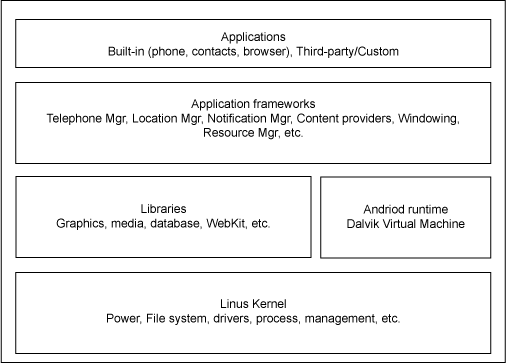
\includegraphics[width=80mm]{img/software_layers.png}}
    \caption{The architecture of the system.}
\end{figure}

Android applications are written in the Java programming language and run within an instance of the Dalvik Virtual Machine.
A key part of the application is the AndroidManifest\@.xml file containing installation meta-data, including the permissions needed to run.
An example of such permission is the ability to use the phone's camera or to access the Internet.
We concentrate more on activities and their development in the following sections. \todo{O aktivitach jsem zatim nic nerekli. Proc ted rikame ctenari, ze se na ne vic zamerime v dalsi sekci?}
\begin{figure}[h!]
    \centering{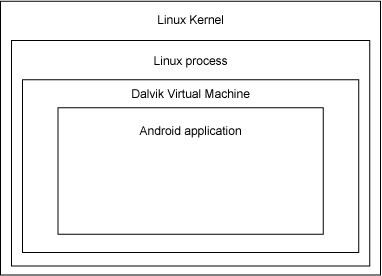
\includegraphics[width=80mm]{img/dalvik.png}}
    \caption{A typical Android application runs within an instance of the Dalvik Virtual Machine.}
\end{figure}

The tools required for the development of an Android application are the Android Software Development Kit (SDK) and a Java IDE, such as Eclipse\footnote{\url{http://www.eclipse.org}} or the Android Studio\footnote{\url{http://developer.android.com/sdk/installing/studio.html}} based on IntelliJ IDEA. 
The Android SDK contains an Eclipse plugin supporting Android developement, documentation, sample code, and various tools, such as Android Debug Bridge used by the programmer to communicate with an application running on a device. 
% % \item The Android SDK is provided as \@.zip file including Java archive file containing all necessary classes to build an application (android\@.jar),
% the SDK documentation, a directory with sample code, Android Debug Bridge and other tools needed to build an application.

% TODO: tohle pripadne pridejme az ten text bude vyladenejsi: In the rest of this chapter we describe some of the implementing parts when developing an application.

\section{Application components}

When an application is installed to a device, it lives within its security sandbox.
Android offers a secure environment where the applications are isolated and can safely run their code.
To each application the Linux system assigns a user ID number. 
Android is a multi-user operating system, meaning that each application corresponds to a different user with a different ID.
This number is known only to the system that sets permissions to all files so they cannot be accessed by any other applications.
Each application runs in a unique Linux process initiated when the application or any of its components need to be executed.
When the system needs to recover the memory or the application is not used for some time, the process shuts down.
Releasing memory is governed by the ``oldest first`` principle -- the system starts by killing the apps that were inactive for the longest time.

The security is driven by the principle of least privilege and the application is allowed access only to the resources specified in the manifest file. 
This protects the whole Android system and the applications from each other.

A typical application is built from several components. 
These basic building blocks can be divided into four different groups:
\begin{itemize}
\item{activities,}
\item{services,}
\item{content providers,}
\item{broadcast receivers.}
\end{itemize}

\emph{An activity} is can be thought of as a UI screen providing elements such as views, lists, buttons, labels, etc. along with the implementation of their functionality.
The layout of an activity and the widgets placed in the window is described in a separate XML file (we reveal more about user interface later) \todo{Tu zavorku rozhodne nahradme odkazem na sekci}
Most applications consist of more than one activity.
Although the activities form one application, they are all independent from each other.
If another application has a permission to do so, it can start an activity of a different app.

Usually in a application there is a one main activity that shows up to the user at first after launching it.
To this one are all other activities linked.
Each activity in android will be subclass of Activity class defined in Android SDK.

A \emph{service} is a component used to perform operations in background.
It can be invoked by an activity for example.
If the application needs to run long-term process, user can switch to another application and our process can continue to run in background.
This can be exploited to develop an application to play music or an application which needs to fetch data in the background.

A \emph{content provider} manages sharing data across the applications.
When the app is storing any data - in file system, SQLite database or any online storage, through the content provider they can be accessed or even modified from other applications.
An example when a content provider is used is an application working with the contacts database.

A \emph{broadcast receiver} is a component broadcasted by the Android system.
It usually inform applications about some basic actions such as turning the screen off, running out of battery or changes of timezone.
Applications can also initiate broadcasts to let other apps know about some action, that there some data ready to use or about completed downloading for example.
%A broadcast receiver is implemented as a subclass of an abstract class BroadcastReceiver.

From these mentioned components, activities, services and broadcasts are activated by intents.
An intent is a message to the system to invoke new activity, service or a broadcast.
It is a component activating mechanism in Android.

A very important part of an application is AndroidManifest\@.xml file, where are specified all permissions of the application.
Each activity we create must be defined in it. Basically, every component that is used in the application must be declared in the manifest.
%code example


\section{The Activity Lifecycle}
\label{sec:lifecycle}

%As we have already stated, a typical application consists of one or more activities.
Any application switches between different states of its life cycle. 
\update{jak souvisi to, ze aplikace ma aktivity s tim, ze aplikace prechazi mezi nejakymi stavy? V dalsim se pak hovori stavech aktivit a ne aplikaci}{}
Compared to desktop platforms, the programmer has only limited control over the state transitions.
\update{napsat priklad toho, co se muze stat na Androidu a nemuze se stat na desktopu}{On the desktop computer we can handle minimalizing or closing a window of an application or quit the entire app. This we can not affect on the Android device.}
The life cycle is a collection of functions operating system calls on the application while it is running.

There are five stages of the life of an application:
\begin{itemize}
\item the starting state,
\item the running state,
\item the paused state,
\item the stopped state,
\item and the destroyed state.
\end{itemize}

The starting state and the destroyed state are phases of the activity when it is not in the memory.
To launch the app, the method \emph{onCreate()} is called and eventually it is in a running state.
When the activity is in a running state it is actually on the screen seen by the user.
The activity is in foreground and handling all user interactions such as typing or touching the screen.
An activity in this state has the highest priority of getting memory in the Android Activity stack to run as quickly as possible.
It will be killed by the operating system only in extreme situations.
This transition from starting to running state is the most expensive operation in terms of battery requirements.
That is also the reason why we do not destroy every activity when it gets to the background, 
because it is probable that it is going to be called back in a while and we don't want to create all of it again.

\begin{figure}[h!]
    \centering{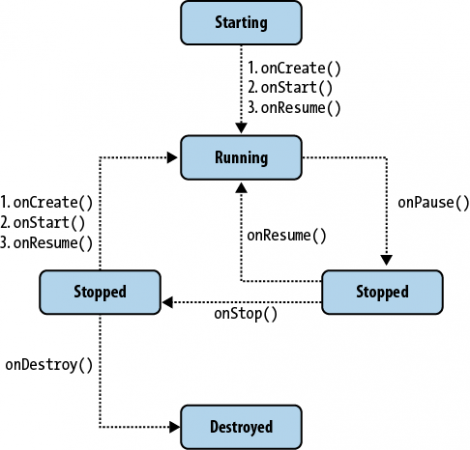
\includegraphics[width=80mm]{img/life_cycles.png}}
    \caption{Life cycles of an application.}
\end{figure}

The application is paused (in a paused state) when it is not interacting with user at the moment, but still visible on the screen.
This state does not occur that often, because most of applications cover entire screen.
But when a dialog box appears or another activity is on the top of this one but not hiding it all, the underlying activity is partly visible and it is paused.

When the application is not visible, but still in memory, it is in a stopped state.
Then it is easy to bring it up to the front again or it can be destroyed, removed from the memory a brought to the destroyed state.

\update{Pribyly nasledujici sekce - User Interface, Sensors a Data Storage}{}



\section{User Interface}
\label{sec:ui}

The user interface is part and parcel of an Android application.
Basically, an application can not live without the user interface.

All elements of the user interface are built using \term{View} or \term{ViewGroup} objects.
By using them we also define the hierarchy of used components - a \term{View} can be nested within a different \term{View}.
The layout describing the visual structure of the \term{Views} of the user interface is declared in separate XML file.
Each \term{View} is represented as a XML element in it corresponding to the View class or subclass.
The user interface can be declared also right in the code of an application. 
Defining it separately make the user interface more flexible to changes without any modification of the code though.
Also, the structure of XML corresponds to the structure of UI and makes it more inspectional and easier to debug.
In the XML file declaring layout can be only one root element. 
It must be a \term{View} or \term{ViewGroup} which is \term{LinearLayout} or \term{RelativeLayout} for example.
\term{LinearLayout} is a layout that arranges the inner elements in a single row or a column depending on the set orientation, 
while in \term{RelativeLayout} are positions of its children described in relation to parent or each other.

The developer tools for Android gives us an option of creating other parts of UI beside sketching the layout such as \term{Menus}, \term{Action Bars}, \term{Dialogs} or \term{Toasts}.
There are several types of \term{Menus} such as \term{options menu} or \term{context menu}.
The \term{options menu} is an user interface component commonly used in many applications collecting menu items for an activity.
It appears when a user touches the menu button.
From the Android version 3\@.0 higher, options menu items are part of the action bar after touching the action overflow button.
The \term{context menu} is a floating menu associated with an particular element in a view that is displayed after touching the element.

\term{Action Bars} are a proper way how to navigate the user through the application.
The \term{Action Bar} is located at the top of an activity and can display the activity title, icon or other actions and items.
Some Android devices have a hardware action overflow button which opens the \term{options menu} at the bottom of an activity (as we mentioned above).
\term{Action Bars} are superiors to \term{options menus} since an \term{Action Bar} is always visible while \term{options menu} shows only on the user request.

\term{Dialog} is a small window informing the user about some action. 
Unlike the \term{Toast} it usually requires the users action before continue by confirmation or giving some additional information.
The \term{Toast} provides only feedback about some action in a small popup that disappears after a moment.


\section{Sensors}

Most Android devices have build in motion, environmental and position sensors.
Motion sensors are sensors measuring rotation along three axes and give us an opportunity to detect motion, shaking or tilt.
For measuring temperature, illumination, or humidity we use environmental sensors.
Build-in magnetometers and orientation sensors provides information about current position of a device and can be used in application for GPS navigation or map browsers.
We can access sensor events within an instance of  the \term{SensorManager} class.

\section{Data Storage}

We have several possibilities how to store our application data.
The way we choose depends on the needs and the level of privacy.
If we use private files in the application and do not want other application to access them, we prefer using the internal storage.
We read and write private data simply by using \term{FileOutputStream} and \term{FileInputStream}.

The media files such as pictures, video or audio records are usually expected to be shared and accessible from other applications.
In that case the external storage is used.
These files are readable and can be modified by user.
Methods on the \term{Environment} class provide the access to the external storage.
The function \term{getExternalStoragePublicDirectory()} depending on the argument given to it returns the path of the root directory where we can write our data, for example

\begin{itemize}
\item{../Music/}
\item{../Pictures/}
\item{../Movies/}
\item{../Download/}
\item{etc.}
\end{itemize}

As an argument we pass the type of the director we want to access, for example \term{Environment\@.DIRECTORYMUSIC}, \term{Environment. DIRECTORYPICTURES}, or \term{Environment. DIRECTORYMUSIC}. %todo: nepodarilo se mi napsat spravne typy jako"DIRECTORY_MUSIC" apod.


\section{Developing Android Application}

In this section we give an outline of implementing the bases for an Android application.

When developing an Android application usually we need to define some user interface.
Some of the components of the UI are described in section \ref{sec:ui}.
The layout of all components is defined in a .xml file.
All .xml files are stored in \term{/res/layout} directory.

The file consists of one root and other descendant xml elements.
Each element is described by the inner attributes of it.
We can see an example of such layout below.
  

\begin{lstlisting}
<?xml version="1.0" encoding="utf-8"?>
<RelativeLayout xmlns:android="http://schemas.android.com/apk/res/android"
    xmlns:tools="http://schemas.android.com/tools"
    android:layout_width="match_parent"
    android:layout_height="match_parent" >

    <org.opencv.android.NativeCameraView
        android:id="@+id/camera_view"
        android:layout_width="match_parent"
        android:layout_height="match_parent" />
    
    <RelativeLayout
	    android:layout_width="200dp"
	    android:layout_height="match_parent"
	    android:layout_margin="10dp"
	    android:layout_centerInParent="true">
	    
        <Button
	        android:id="@+id/captureButton"
	        android:layout_width="90dp"
	        android:layout_height="90dp"
	        android:layout_alignParentBottom="true"
	        android:layout_centerHorizontal="true"
	        android:background="@drawable/circle_button"
	        android:onClick="callTakePicture"/>
        
        <Button
	        android:id="@+id/startCapturingButton"
	        android:layout_width="90dp"
	        android:layout_height="90dp"
	        android:layout_alignParentBottom="true"
	        android:layout_centerHorizontal="true"
	        android:background="@drawable/circle_button"
	        android:onClick="start_stopAutoCapturing"
	        android:visibility="invisible"/>
	          
	    <ToggleButton
	        android:id="@+id/toggleAutoCaptureButton"
              android:layout_width="wrap_content" 
              android:layout_height="wrap_content" 
              android:layout_alignParentTop="true"
              android:layout_centerHorizontal="true"
	        android:textOn="AutoCapture on"
	        android:textOff="AutoCapture off"	    
	        android:onClick="autoCaptureStateChanged"/>

	    <TextView
	        android:id="@+id/startCapturing_textView"
	        android:layout_width="wrap_content"
	        android:layout_height="wrap_content"
	        android:layout_above="@+id/captureButton"
	        android:layout_centerHorizontal="true"
	        android:text="@string/startcapturing_text"
	        android:visibility="invisible"/>

	</RelativeLayout>
	
</RelativeLayout>

\end{lstlisting}

In our example the root element is \term{RelativeLayout} element which allows us to describe the relative position to each other or to a parent.
Inside the \term{RelativeLayout} we can find \term{org.opencv.android.NativeCameraView} which is an element of OpenCV library used for camera view and 
another \term{RelativeLayout} with \term{Buttons},  a \term{ToggleButton} and a \term{TextView}.
All of the elements have defined the width an height by using \term{android:layoutwidth} and \term{android:layoutwidth} attributes.
The value of these attributes can be \term{matchparent}or \term{wrapcontent} or the specific number of dp units.

It is also possible to define different layout of one activity depending on the screen orientation.
If we need to define different layout for landscape orientation, we save a xml file of the same name with new layout into \term{res/layout-land} folder.

In the \term{src} folder are stored all .java files representing activities or classes.
Every Android application has at least one activity which is called by the system when the application is launched.
Due to the activity lifecycle (see \ref{sec:lifecycle}) it is necessary to implement the following methods:

\begin{itemize}
\item \term{onCreate()},
\item \term{onPause()},
\item \term{onResume()}.
\end{itemize}

The \term{onCreate()} method handles what happens when the activity is started.
Usually only the basic startup instructions should be completed in this method, for example setting the layout or initialisation of some class variables.
The particular layout into an activity is loaded by \term{setContentView(name-of-the-xml-file)}.
We can see an example of \term{onCreate()} method below.

\begin{lstlisting}
    @Override
    public void onCreate(Bundle savedInstanceState) {
        super.onCreate(savedInstanceState);
        setContentView(R.layout.activity_gallery);
        
        adapter = new Adapter(this);
        ArrayList<GridImage> db_update = new ArrayList<GridImage>();
        for (String s : files) {
          ...
        }
        ...
  }
\end{lstlisting}

Depending on the needs of our application, we can add some code into the other overriding methods handling the activity lifecycle.

\begin{lstlisting}
  
  @Override
  public void onPause(){
      super.onPause();
      ...
  }
	
  @Override
  public void onResume(){
      super.onResume();
      ...
  }
      
\end{lstlisting}

To make our user interface interactive we need to set some functions that will be executed when clicking on the elements of the user interface.
This can be done either in the xml file or in the code of the activity.
To demonstrate these two approaches, we added an example:

\begin{lstlisting}
/* This is the definition of a button in the xml file. 
    When clicking on the button, takePicture() method will be executed.
    The method must be defined in the .java file of the activity. */
<Button  
  ...
  android:onClick="takePicture"
  ... />
  
/* This is the example how to define 
    the method directly in the code. */

Button my_button = (Button)findViewById(R.id.button);
my_button.setOnClickListener( new View.OnClickListener() {
    
});
  
 
  
\end{lstlisting}









